\chapter{Requirements}
%I dette afsnit beskrives krav til systemet med en kort beskrivelse af aktører, de vigtigste use-cases (funktionelle krav) og de vigtigste ikke-funktionelle krav. Beskrivelserne bør referere til kravspecifikationen i projektets bilag for yderligere detaljer. Ikke-funktionelle krav skal beskrives overordnet uden specifikke detaljer som f.eks. krav til værdier og nøjagtigheder, her henvises igen til kravspecifikationen i projektets bilag.
To get a sense of the system and what requirements the system should have, some mock-ups of a user interface were created and can be found in the documentation in section~\ref{sec:mockups} on page~\pageref{sec:mockups}.

\begin{figure}[H]
\centering
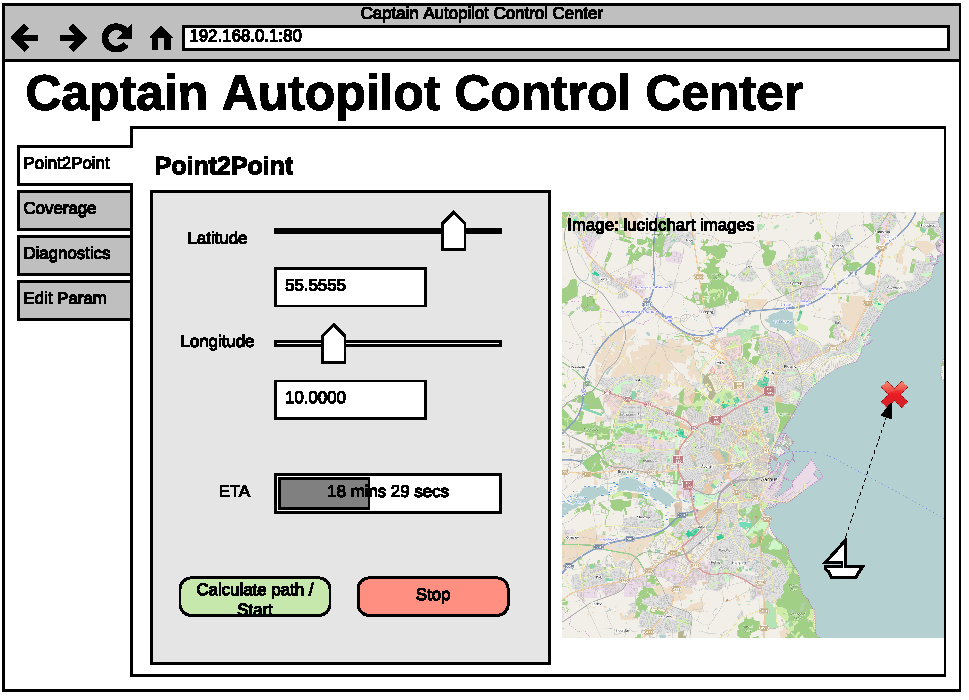
\includegraphics[width=0.7\linewidth]{../Appendix/Project/Dokumentation/Images/Requirements_specification/UI_Mockup_Point_to_point}
\caption{Mockup for the Point to point menu}
\label{fig:uimockuppointtopoint}
\end{figure}

An example of one of these mock-ups, describing a waypoint to navigate towards, can be seen in figure~\ref{fig:uimockuppointtopoint}. It describes how the a user should interact with the system, and how the system should communicate with the user.

To describe the functionality in further detail, a use case driven approach has been used. First of all, the actors of the system have to be identified. In figure~\ref{fig:uimockuppointtopoint} is the use case diagram for the system, on the left are the actors that initiate a use case, and on the right is the secondary actors, in this case the GPS receiver.

The initiating, or primary, actors of the CAPTAIN system are a technician and a user. The technician is an actor who sets up the system, and has a more in-depth knowledge of the system than the user. The user could be anyone, since all of the complicated work should be handled by the system or the technician. 

\begin{figure}[H]
\centering
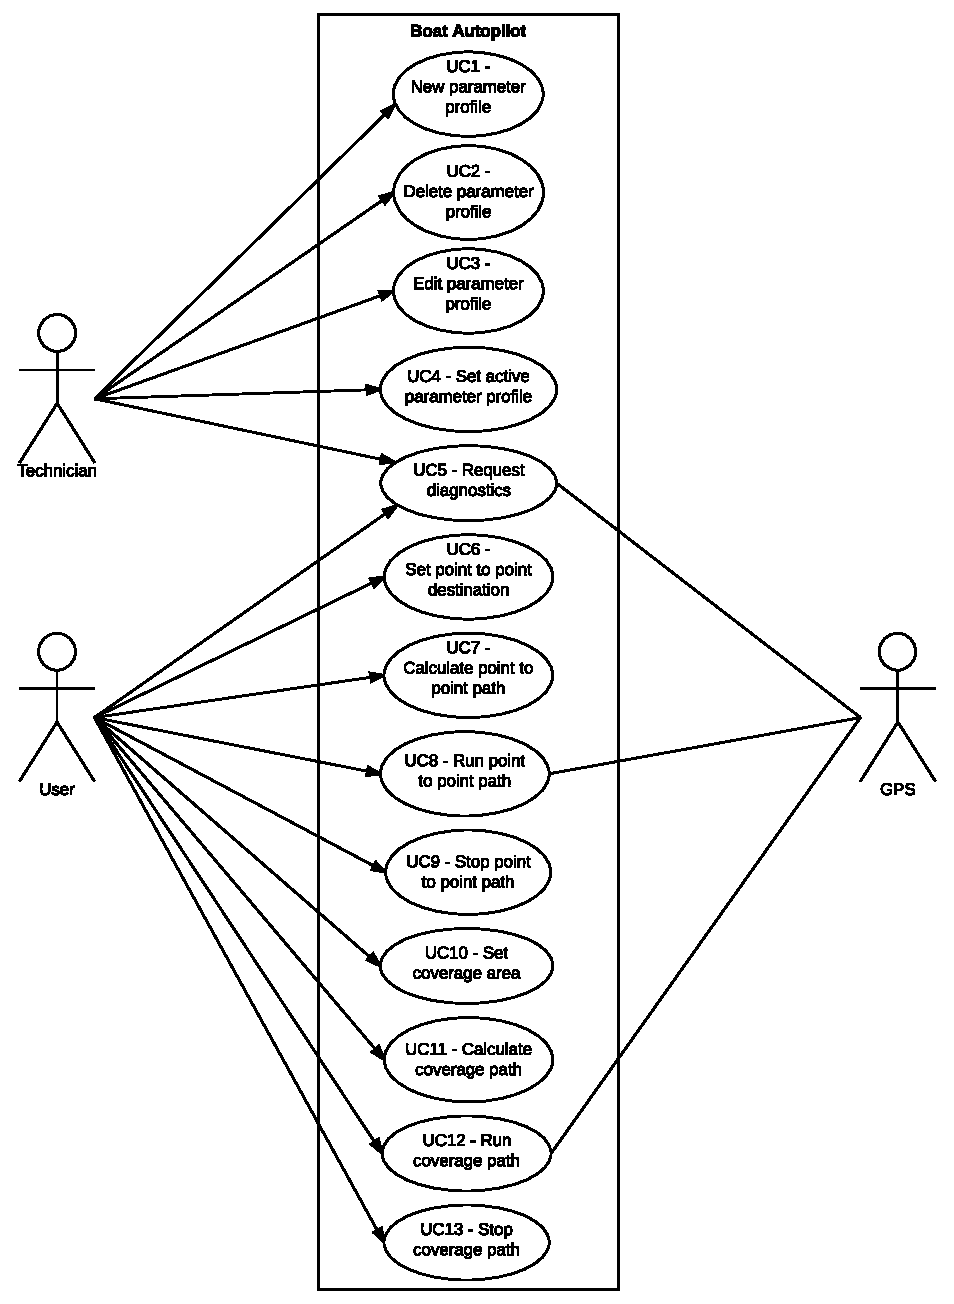
\includegraphics[max width =1\linewidth]{../Appendix/Project/Dokumentation/Images/Requirements_specification/Usecase_diagram}
\caption{Use case diagram}
\label{fig:usecasediagram}
\end{figure}

The use case diagram on figure~\ref{fig:usecasediagram} lists 13 different use cases. A use case describes a way to use the system. In this system they mainly describe a button or function that can be started by the user. In this section a few use cases will be looked at, but for all the fully dressed use cases, one can have a look at the documentation section ~\ref{sec:usecases} on page~\pageref{sec:usecases}.

\section{Use case 3 - Edit parameter profile}
One of the first things that was realized the system needed, was a way to describe and modify the parameters of the system. Parameters could be PID-loop terms, or the size of the boat, in fact anything that could be of use to the system. So to be able to save these parameters, parameter profiles were introduced. A parameter profile is essentially a list of any kind of parameters. Use case 3 - "Edit parameter profile", is the use case used to change the values of an already created parameter profile. It's important to note that it is the technician who initiates this use case, since he knows exactly what the values should be, and this requires some deeper knowledge of the system. 

\section{Use case 11 - Calculate coverage path}
There are many ways to navigate waypoints, first of all one needs to decide on how to describe the waypoints. For this system, waypoints are used in two ways; either as a single point to reach, or as a rectangle to cover. For the rectangle, the system should calculate a path that covers a the rectangle with lines that have a predefined distance between them. This use case should be initialized by the user, with a simple click in the user interface. In return the user interface should display the calculated path, so the user can tell if the path is what they wanted.

\section{Use case 12 - Run coverage path}
With a calculated path, i.e. a list of waypoints to follow, the boat should be able to traverse these points. When the user presses the button labeled "Run", Use case 12 - "Run coverage path" is initiated, and it should not finish until the boat has reached the last waypoint of the list of waypoints. The boat should get through the waypoints using a control loop. While the boat is running, an estimated time enroute should be displayed along with the current position of the boat.

\section{Use case 5 - Request diagnostics}
At any point in time, it may be convenient for the user or the technician to have access to information about the boat. In other words, getting the diagnostics data from the boat. Diagnostics data might include GPS information, what position the rudder is set to and so forth. This use case can, as mentioned, be initiated by either the user or the technician, by the press of a button in the user interface. 



